% !TEX root =  ./main.tex

\section{Auxiliary Material}

\subsection{Auxiliary Material for the toy running example}

The \BioResolve specification for the toy running example about the interaction between the student and the vending machine is reported in \Cref{fig:bioresolve:toy}. The corresponding RS has been described in \Cref{sec:student} and it has been used to illustrate some key features of the \GROOVE encoding in \Cref{sec:RS2GTS}.

\begin{figure}[t]
\begin{minipage}{0.9\linewidth}
\footnotesize
\begin{verbatim}
myentities([cpowder,tpowder]). % initial set D0

myreactions([                  % list of reactions
    react([idle],[am],[am]),
    react([am],[idle],[am]),
    react([ccoin,cpowder],[nomilk],[cappuccino]),
    react([ccoin,cpowder,nomilk],[],[espresso]),
    react([tcoin,tpowder],[],[tea]),
    react([cpowder],[],[cpowder]),
    react([tpowder],[],[tpowder]),
    react([anger],[],[bang]) ]).

mycontext("[refill,student]"). % context processes

myenvironment("[               % context definitions
    refill = ({nomilk}.refill 
            + {}.refill),
    student = (?{},{am},{tcoin}?.gettea 
             + ?{am},{},{ccoin}?.getcappuccino 
             + {idle}.student),
    gettea = (?{tea},{},{}?.student
            + ?{},{tea},{anger}?.student),
    getcappuccino = (?{cappuccino},{},{}?.student 
                    + ?{espresso},{},{anger}?.student) ]").
\end{verbatim}
\end{minipage}
\caption{\BioResolve implementation of the vending machine RS from \Cref{sec:student}.}
\label{fig:bioresolve:toy}
\end{figure}

\subsection{Auxiliary Material for the Comorbidity Case Study}

The \BioResolve specification for the comorbidity case study presented in~\cite{DBLP:conf/cmsb/BowlesBBFGM24} is reported in \Cref{fig:bioresolve:comorbidities}. The corresponding experimentation with \GROOVE has been discussed in \Cref{sec:cmsb2024}.

\begin{figure*}[t]
\fontsize{6}{0}
\[
\begin{array}{rcl}
\mathsf{D}_0 & \triangleq & \varnothing
\\[-4pt]
\mathsf{Feats} &  \triangleq 
& (\{\mathsf{hyper}\},\varnothing,\{\mathsf{hyper}\})
\mid  (\{\mathsf{afib}\},\varnothing,\{\mathsf{afib}\})
\mid  (\{\mathsf{has\_fib}\},\varnothing,\{\mathsf{has\_fib}\})
\mid  (\{\mathsf{heart\_rate}\},\varnothing,\{\mathsf{heart\_rate}\})
\mid  (\{\mathsf{consensus\_acei}\},\varnothing,\{\mathsf{consensus\_acei}\})
\\[-4pt] & \mid &  (\{\mathsf{over75}\},\varnothing,\{\mathsf{over75}\})
\mid  (\{\mathsf{below55}\},\varnothing,\{\mathsf{below55}\})
\mid  (\{\mathsf{diabete}\},\varnothing,\{\mathsf{diabete}\})
\mid  (\{\mathsf{origin}\},\varnothing,\{\mathsf{origin}\})
\\[-4pt] & \mid &  (\{\mathsf{doac\_int}\},\varnothing,\{\mathsf{doac\_int}\})
\mid  (\{\mathsf{hyper}\},\varnothing,\{\mathsf{diseases}\})
\mid  (\{\mathsf{diabete}\},\varnothing,\{\mathsf{diseases}\})
\\[-4pt]
\mathsf{Drugs} &  \triangleq 
& (\{\mathsf{get\_diltiazem}\},\{\mathsf{stop\_cbb}\},\{\mathsf{diltiazem},\mathsf{cbb}\})
\mid  (\{\mathsf{diltiazem}\},\{\mathsf{stop\_cbb}\},\{\mathsf{diltiazem},\mathsf{cbb}\})
\mid  (\{\mathsf{get\_verapamil}\},\{\mathsf{stop\_cbb}\},\{\mathsf{verapamil},\mathsf{cbb}\})
\\[-4pt] & \mid &  (\{\mathsf{verapamil}\},\{\mathsf{stop\_cbb}\},\{\mathsf{verapamil},\mathsf{cbb}\})
\mid  (\{\mathsf{diltiazem},\mathsf{verapamil}\},\{\mathsf{stop\_cbb}\},\{\mathsf{alert\_dup}\})
%
\mid  (\{\mathsf{get\_propranolol}\},\{\mathsf{stop\_nsbb}\},\{\mathsf{propranolol},\mathsf{nsbb}\})
\\[-4pt] & \mid &  (\{\mathsf{propranolol}\},\{\mathsf{stop\_nsbb}\},\{\mathsf{propranolol},\mathsf{nsbb}\})
\mid  (\{\mathsf{get\_carvedilol}\},\{\mathsf{stop\_nsbb}\},\{\mathsf{carvedilol},\mathsf{nsbb}\})
\mid  (\{\mathsf{carvedilol}\},\{\mathsf{stop\_nsbb}\},\{\mathsf{carvedilol},\mathsf{nsbb}\})
\\[-4pt] & \mid &  (\{\mathsf{propranolol},\mathsf{carvedilol}\},\{\mathsf{stop\_nsbb}\},\{\mathsf{alert\_dup}\})
%
\mid  (\{\mathsf{get\_bisoprolol}\},\{\mathsf{stop\_sbb}\},\{\mathsf{bisoprolol},\mathsf{sbb}\})
\mid  (\{\mathsf{bisoprolol}\},\{\mathsf{stop\_sbb}\},\{\mathsf{bisoprolol},\mathsf{sbb}\})
\\[-4pt] & \mid &  (\{\mathsf{get\_atenolol}\},\{\mathsf{stop\_sbb}\},\{\mathsf{atenolol},\mathsf{sbb}\})
\mid  (\{\mathsf{atenolol}\},\{\mathsf{stop\_sbb}\},\{\mathsf{atenolol},\mathsf{sbb}\})
\mid  (\{\mathsf{bisoprolol},\mathsf{atenolol}\},\{\mathsf{stop\_sbb}\},\{\mathsf{alert\_dup}\})
%
\\[-4pt] & \mid &  (\{\mathsf{get\_flecainide}\},\{\mathsf{stop\_flec}\},\{\mathsf{flecainide}\})
\mid  (\{\mathsf{flecainide}\},\{\mathsf{stop\_flec}\},\{\mathsf{flecainide}\})
\mid  (\{\mathsf{get\_warfarin}\},\{\mathsf{stop\_warf}\},\{\mathsf{warfarin}\})
\\[-4pt] & \mid &  (\{\mathsf{warfarin}\},\{\mathsf{stop\_warf}\},\{\mathsf{warfarin}\})
%
\mid  (\{\mathsf{get\_apixaban}\},\{\mathsf{stop\_doac}\},\{\mathsf{apixaban},\mathsf{doac}\})
\mid  (\{\mathsf{apixaban}\},\{\mathsf{stop\_doac}\},\{\mathsf{apixaban},\mathsf{doac}\})
\\[-4pt] & \mid &  (\{\mathsf{get\_dabigatran}\},\{\mathsf{stop\_doac}\},\{\mathsf{dabigatran},\mathsf{doac}\})
\mid  (\{\mathsf{dabigatran}\},\{\mathsf{stop\_doac}\},\{\mathsf{dabigatran},\mathsf{doac}\})
\mid  (\{\mathsf{apixaban},\mathsf{dabigatran}\},\{\mathsf{stop\_doac}\},\{\mathsf{alert\_dup}\})
%
\\[-4pt] & \mid &  (\{\mathsf{get\_vkant}\},\{\mathsf{stop\_vkant}\},\{\mathsf{vkant}\})
\mid  (\{\mathsf{vkant}\},\{\mathsf{stop\_vkant}\},\{\mathsf{vkant}\})
%
\mid  (\{\mathsf{get\_benazepril}\},\{\mathsf{stop\_acei}\},\{\mathsf{benazepril},\mathsf{acei}\})
\\[-4pt] & \mid &  (\{\mathsf{benazepril}\},\{\mathsf{stop\_acei}\},\{\mathsf{benazepril},\mathsf{acei}\})
\mid  (\{\mathsf{get\_captopril}\},\{\mathsf{stop\_acei}\},\{\mathsf{captopril},\mathsf{acei}\})
\mid  (\{\mathsf{captopril}\},\{\mathsf{stop\_acei}\},\{\mathsf{captopril},\mathsf{acei}\})
\\[-4pt] & \mid &  (\{\mathsf{benazepril},\mathsf{captopril}\},\{\mathsf{stop\_acei}\},\{\mathsf{alert\_dup}\})
%
\mid  (\{\mathsf{get\_olmesortan}\},\{\mathsf{stop\_arb}\},\{\mathsf{olmesortan},\mathsf{arb}\})
\mid  (\{\mathsf{olmesortan}\},\{\mathsf{stop\_arb}\},\{\mathsf{olmesortan},\mathsf{arb}\})
\\[-4pt] & \mid &  (\{\mathsf{get\_irbesartan}\},\{\mathsf{stop\_arb}\},\{\mathsf{irbesartan},\mathsf{arb}\})
\mid  (\{\mathsf{irbesartan}\},\{\mathsf{stop\_arb}\},\{\mathsf{irbesartan},\mathsf{arb}\})
\mid  (\{\mathsf{olmesortan},\mathsf{irbesartan}\},\{\mathsf{stop\_arb}\},\{\mathsf{alert\_dup}\})
%
\\[-4pt] & \mid &  (\{\mathsf{get\_indapamide}\},\{\mathsf{stop\_td}\},\{\mathsf{indapamide},\mathsf{td}\})
\mid  (\{\mathsf{indapamide}\},\{\mathsf{stop\_td}\},\{\mathsf{indapamide},\mathsf{td}\})
\mid  (\{\mathsf{get\_chlorothiazide}\},\{\mathsf{stop\_td}\},\{\mathsf{chlorothiazide},\mathsf{td}\})
\\[-4pt] & \mid &  (\{\mathsf{chlorothiazide}\},\{\mathsf{stop\_td}\},\{\mathsf{chlorothiazide},\mathsf{td}\})
\mid  (\{\mathsf{indapamide},\mathsf{chlorothiazide}\},\{\mathsf{stop\_td}\},\{\mathsf{alert\_dup}\})
%
\mid  (\{\mathsf{doac}\},\{\mathsf{doac\_ok},\mathsf{doac\_fail}\},\{\mathsf{doac\_test}\})
\\[-4pt] & \mid &  (\{\mathsf{doac\_ok}\},\{\mathsf{doac\_fail}\},\{\mathsf{doac\_ok}\})
\mid  (\{\mathsf{doac\_fail}\},\{\mathsf{doac\_ok}\},\{\mathsf{doac\_fail}\})
\mid  (\{\mathsf{doac}\},\{\mathsf{doac\_fail},\mathsf{stop\_doac}\},\{\mathsf{doac\_danger}\})
\\[-4pt] & \mid &  (\{\mathsf{doac}\},\{\mathsf{doac\_danger},\mathsf{stop\_doac}\},\{\mathsf{danger}\})
\\[-4pt]
\mathsf{ADR} &  \triangleq 
& (\{\mathsf{get\_apixaban},\mathsf{get\_diltiazem}\},\varnothing,\{\mathsf{moderate}\})
\mid  (\{\mathsf{get\_apixaban},\mathsf{diltiazem}\},\varnothing,\{\mathsf{moderate}\})
\mid  (\{\mathsf{apixaban},\mathsf{get\_diltiazem}\},\varnothing,\{\mathsf{moderate}\})
\\[-4pt] & \mid &  (\{\mathsf{apixaban},\mathsf{diltiazem}\},\varnothing,\{\mathsf{moderate}\})
\mid  (\{\mathsf{get\_apixaban},\mathsf{get\_verapamil}\},\varnothing,\{\mathsf{moderate}\})
\mid  (\{\mathsf{get\_apixaban},\mathsf{verapamil}\},\varnothing,\{\mathsf{moderate}\})
\\[-4pt] & \mid &  (\{\mathsf{apixaban},\mathsf{get\_verapamil}\},\varnothing,\{\mathsf{moderate}\})
\mid  (\{\mathsf{apixaban},\mathsf{verapamil}\},\varnothing,\{\mathsf{moderate}\})
\mid  (\{\mathsf{get\_dabigatran},\mathsf{get\_diltiazem}\},\varnothing,\{\mathsf{moderate}\})
\\[-4pt] & \mid &  (\{\mathsf{get\_dabigatran},\mathsf{diltiazem}\},\varnothing,\{\mathsf{moderate}\})
\mid  (\{\mathsf{dabigatran},\mathsf{get\_diltiazem}\},\varnothing,\{\mathsf{moderate}\})
\mid  (\{\mathsf{dabigatran},\mathsf{diltiazem}\},\varnothing,\{\mathsf{moderate}\})
\\[-4pt] & \mid &  (\{\mathsf{get\_dabigatran},\mathsf{get\_verapamil}\},\varnothing,\{\mathsf{major}\})
\mid  (\{\mathsf{get\_dabigatran},\mathsf{verapamil}\},\varnothing,\{\mathsf{major}\})
\mid  (\{\mathsf{dabigatran},\mathsf{get\_verapamil}\},\varnothing,\{\mathsf{major}\})
\\[-4pt] & \mid &  (\{\mathsf{dabigatran},\mathsf{verapamil}\},\varnothing,\{\mathsf{major}\})
\mid  (\{\mathsf{get\_dabigatran},\mathsf{get\_carvedilol}\},\varnothing,\{\mathsf{moderate}\})
\mid  (\{\mathsf{get\_dabigatran},\mathsf{carvedilol}\},\varnothing,\{\mathsf{moderate}\})
\\[-4pt] & \mid &  (\{\mathsf{dabigatran},\mathsf{get\_carvedilol}\},\varnothing,\{\mathsf{moderate}\})
\mid  (\{\mathsf{dabigatran},\mathsf{carvedilol}\},\varnothing,\{\mathsf{moderate}\})
\mid  (\{\mathsf{get\_warfarin},\mathsf{get\_benazepril}\},\varnothing,\{\mathsf{minor}\})
\\[-4pt] & \mid &  (\{\mathsf{get\_warfarin},\mathsf{benazepril}\},\varnothing,\{\mathsf{minor}\})
\mid  (\{\mathsf{warfarin},\mathsf{get\_benazepril}\},\varnothing,\{\mathsf{minor}\})
\mid  (\{\mathsf{warfarin},\mathsf{benazepril}\},\varnothing,\{\mathsf{minor}\})
\\[-4pt] & \mid &  (\{\mathsf{get\_warfarin},\mathsf{get\_indapamide}\},\varnothing,\{\mathsf{minor}\})
\mid  (\{\mathsf{get\_warfarin},\mathsf{indapamide}\},\varnothing,\{\mathsf{minor}\})
\mid  (\{\mathsf{warfarin},\mathsf{get\_indapamide}\},\varnothing,\{\mathsf{minor}\})
\\[-4pt] & \mid &  (\{\mathsf{warfarin},\mathsf{indapamide}\},\varnothing,\{\mathsf{minor}\})
\mid  (\{\mathsf{get\_warfarin},\mathsf{get\_chlorothiazide}\},\varnothing,\{\mathsf{minor}\})
\mid  (\{\mathsf{get\_warfarin},\mathsf{chlorothiazide}\},\varnothing,\{\mathsf{minor}\})
\\[-4pt] & \mid &  (\{\mathsf{warfarin},\mathsf{get\_chlorothiazide}\},\varnothing,\{\mathsf{minor}\})
\mid  (\{\mathsf{warfarin},\mathsf{chlorothiazide}\},\varnothing,\{\mathsf{minor}\})
\mid  (\{\mathsf{get\_warfarin},\mathsf{get\_propranolol}\},\varnothing,\{\mathsf{minor}\})
\\[-4pt] & \mid &  (\{\mathsf{get\_warfarin},\mathsf{propranolol}\},\varnothing,\{\mathsf{minor}\})
\mid  (\{\mathsf{warfarin},\mathsf{get\_propranolol}\},\varnothing,\{\mathsf{minor}\})
\mid  (\{\mathsf{warfarin},\mathsf{propranolol}\},\varnothing,\{\mathsf{minor}\})
\\[-4pt] & \mid &  (\{\mathsf{get\_flecainide},\mathsf{get\_diltiazem}\},\varnothing,\{\mathsf{major}\})
\mid  (\{\mathsf{get\_flecainide},\mathsf{diltiazem}\},\varnothing,\{\mathsf{major}\})
\mid  (\{\mathsf{flecainide},\mathsf{get\_diltiazem}\},\varnothing,\{\mathsf{major}\})
\\[-4pt] & \mid &  (\{\mathsf{flecainide},\mathsf{diltiazem}\},\varnothing,\{\mathsf{major}\})
\mid  (\{\mathsf{get\_flecainide},\mathsf{get\_verapamil}\},\varnothing,\{\mathsf{major}\})
\mid  (\{\mathsf{get\_flecainide},\mathsf{verapamil}\},\varnothing,\{\mathsf{major}\})
\\[-4pt] & \mid &  (\{\mathsf{flecainide},\mathsf{get\_verapamil}\},\varnothing,\{\mathsf{major}\})
\mid  (\{\mathsf{flecainide},\mathsf{verapamil}\},\varnothing,\{\mathsf{major}\})
\mid  (\{\mathsf{get\_flecainide},\mathsf{get\_bisoprolol}\},\varnothing,\{\mathsf{moderate}\})
\\[-4pt] & \mid &  (\{\mathsf{get\_flecainide},\mathsf{bisoprolol}\},\varnothing,\{\mathsf{moderate}\})
\mid  (\{\mathsf{flecainide},\mathsf{get\_bisoprolol}\},\varnothing,\{\mathsf{moderate}\})
\mid  (\{\mathsf{flecainide},\mathsf{bisoprolol}\},\varnothing,\{\mathsf{moderate}\})
\\[-4pt] & \mid &  (\{\mathsf{get\_flecainide},\mathsf{get\_atenolol}\},\varnothing,\{\mathsf{moderate}\})
\mid  (\{\mathsf{get\_flecainide},\mathsf{atenolol}\},\varnothing,\{\mathsf{moderate}\})
\mid  (\{\mathsf{flecainide},\mathsf{get\_atenolol}\},\varnothing,\{\mathsf{moderate}\})
\\[-4pt] & \mid &  (\{\mathsf{flecainide},\mathsf{atenolol}\},\varnothing,\{\mathsf{moderate}\})
\mid  (\{\mathsf{get\_flecainide},\mathsf{get\_propranolol}\},\varnothing,\{\mathsf{moderate}\})
\mid  (\{\mathsf{get\_flecainide},\mathsf{propranolol}\},\varnothing,\{\mathsf{moderate}\})
\\[-4pt] & \mid &  (\{\mathsf{flecainide},\mathsf{get\_propranolol}\},\varnothing,\{\mathsf{moderate}\})
\mid  (\{\mathsf{flecainide},\mathsf{propranolol}\},\varnothing,\{\mathsf{moderate}\})
\mid  (\{\mathsf{get\_flecainide},\mathsf{get\_carvedilol}\},\varnothing,\{\mathsf{moderate}\})
\\[-4pt] & \mid &  (\{\mathsf{get\_flecainide},\mathsf{carvedilol}\},\varnothing,\{\mathsf{moderate}\})
\mid  (\{\mathsf{flecainide},\mathsf{get\_carvedilol}\},\varnothing,\{\mathsf{moderate}\})
\mid  (\{\mathsf{flecainide},\mathsf{carvedilol}\},\varnothing,\{\mathsf{moderate}\})
\\[-4pt] & \mid &  (\{\mathsf{major}\},\varnothing,\{\mathsf{major}\})
\mid  (\{\mathsf{moderate}\},\varnothing,\{\mathsf{moderate}\})
\mid  (\{\mathsf{minor}\},\varnothing,\{\mathsf{minor}\})
\mid  (\{\mathsf{alert\_dup}\},\varnothing,\{\mathsf{alert\_dup}\})
\mid  (\{\mathsf{danger}\},\varnothing,\{\mathsf{danger}\})
\\[-4pt]
\mathsf{eafib1} &  \triangleq 
& (\varnothing,\{\mathsf{afib}\},\varnothing).\mathsf{eafib1} + (\{\mathsf{afib}\},\varnothing,\varnothing).\mathsf{ehr}
\\[-4pt]
\mathsf{ehr} &  \triangleq 
& (\varnothing,\{\mathsf{heart\_rate}\},\varnothing).\mathsf{ehr} + (\{\mathsf{heart\_rate}\},\varnothing,\varnothing).\mathsf{ebb}
\\[-4pt]
\mathsf{ebb} &  \triangleq 
& \varnothing.\mathsf{ebb} + \mathsf{e\_cbb} + \mathsf{e\_nsbb} + \mathsf{e\_sbb}
\\[-4pt]
\mathsf{e\_cbb} &  \triangleq 
& (\varnothing,\{\mathsf{verapamil}\},\{\mathsf{get\_diltiazem}\}).\mathsf{empty} + (\varnothing,\{\mathsf{diltiazem}\},\{\mathsf{get\_verapamil}\}).\mathsf{empty}
\\[-4pt]
\mathsf{e\_nsbb} &  \triangleq 
& (\varnothing,\{\mathsf{carvedilol}\},\{\mathsf{get\_propranolol}\}).\mathsf{empty} + (\varnothing,\{\mathsf{propranolol}\},\{\mathsf{get\_carvedilol}\}).\mathsf{empty}
\\[-4pt]
\mathsf{e\_sbb} &  \triangleq 
& (\varnothing,\{\mathsf{atenolol}\},\{\mathsf{get\_bisoprolol}\}).\mathsf{empty} + (\varnothing,\{\mathsf{bisoprolol}\},\{\mathsf{get\_atenolol}\}).\mathsf{empty}
\\[-4pt]
\mathsf{eafib2} &  \triangleq 
& (\varnothing,\{\mathsf{afib}\},\varnothing).\mathsf{eafib2} + (\{\mathsf{afib}\},\varnothing,\varnothing).\mathsf{ehf}
\\[-4pt]
\mathsf{ehf} &  \triangleq 
& (\varnothing,\{\mathsf{has\_fib}\},\varnothing).\mathsf{ehf} + (\{\mathsf{has\_fib}\},\varnothing,\varnothing).\mathsf{eflec}
\\[-4pt]
\mathsf{eflec} &  \triangleq 
& \varnothing.\mathsf{eflec} + \mathsf{e\_flec}
\\[-4pt]
\mathsf{e\_flec} &  \triangleq 
& \{\mathsf{get\_flecainide}\}.\mathsf{empty}
\\[-4pt]
\mathsf{eafib3} &  \triangleq 
& (\varnothing,\{\mathsf{afib}\},\varnothing).\mathsf{eafib3} + (\{\mathsf{afib}\},\varnothing,\varnothing).\mathsf{econs}
\end{array}
%myenvironment("[
%  econs = (?{},{heart_rate,has_fib},{}?.econs + ?{},{consensus_acei},{}?.econs 
%           + ?{consensus_acei,heart_rate},{},{}?.estroke + ?{consensus_acei,has_fib},{},{}?.estroke),
%  estroke = (?{},{diseases,over75},{}?.ewarf + ?{over75},{doac_fail,doac_int},{}?.edoac + ?{diseases},{doac_fail,doac_int},{}?.edoac 
%           + ?{over75,doac_fail},{},{}?.evkant + ?{over75,doac_int},{},{}?.evkant + ?{diseases,doac_fail},{},{}?.evkant + ?{diseases,doac_int},{},{}?.evkant),
%  ewarf = ({}.ewarf + e_warf),
%  e_warf = {get_warfarin}.empty,
%  edoac = ({}.edoac + e_doac),
%  e_doac = (?{},{dabigatran},{get_apixaban}?.e_doacfail + ?{},{apixaban},{get_dabigatran}?.e_doacfail),
%  e_doacfail = (?{doac_fail},{},{stop_doac}?.evkant + ?{},{doac_fail},{}?.e_doacfail),
%  evkant = ({}.evkant + e_vkant),
%  e_vkant = {get_vkant}.empty,	
%  ghyper = (?{},{hyper},{}?.ghyper + ?{hyper},{},{}?.g1),
%  g1 = (?{diabete},{},{}?.g2 + ?{below55},{diabete,origin},{}?.g2 + ?{},{below55,diabete},{}?.g3 + ?{origin},{diabete},{}?.g3),
%  g2 = ({}.g2 + <1,e_acei>.g4 + <1,e_arb>.g5),
%  g3 = ({}.g3 + <1,e_cbb>.g6),
%  g4 = ({}.g4 + <1,e_cbb>.g7 + <1,e_td>.g8),
%  g5 = ({}.g5 + <1,e_cbb>.g9 + <1,e_td>.g10),
%  g6 = ({}.g6 + <1,e_acei>.g7 + <1,e_arb>.g9 + <1,e_td>.g11),
%  g7 = ({}.g7 + <1,e_arb>.etd + <1,e_td>.earb),
%  g8 = ({}.g8 + <1,e_arb>.ecbb + <1,e_cbb>.earb),
%  g9 = ({}.g9 + <1,e_acei>.etd + <1,e_td>.eacei),
%  g10 = ({}.g10 + <1,e_acei>.ecbb + <1,e_cbb>.eacei),
%  g11 = ({}.g11 + <1,e_acei>.earb + <1,e_arb>.eacei),
%  ecbb = ({}.ecbb + e_cbb),
%  eacei = ({}.eacei + e_acei),
%  e_acei = (?{},{captopril},{get_benazepril}?.empty + ?{},{benazepril},{get_captopril}?.empty),
%  earb = ({}.earb + e_arb),
%  e_arb = (?{},{irbesartan},{get_olmesortan}?.empty + ?{},{olmesortan},{get_irbesartan}?.empty),
%  etd = ({}.etd + e_td),
%  e_td = (?{},{chlorothiazide},{get_indapamide}?.empty + ?{},{indapamide},{get_chlorothiazide}?.empty),
%  k_doac = (?{doac_test},{},{doac_ok}?.empty + ?{doac_test},{},{doac_fail}?.empty + ?{},{doac_test},{}?.k_doac),
%  empty = {}.empty,
%  kafib = ({afib}.empty + empty),
%  khf = ({has_fib}.empty + empty),
%  khr = ({heart_rate}.empty + empty),
%  kcons = ({consensus_acei}.empty + empty),
%  kage = ({over75}.empty + {below55}.empty + empty),
%  kdiabete = ({diabete}.empty + empty),
%  kdoacint = ({doac_int}.empty + empty),
%  khyper = ({hyper}.empty + empty),
%  korigin = ({origin}.empty + empty) ]"). 
%
%mycontext("[eafib1,eafib2,eafib3,ghyper,kafib,khf,khr,kcons,kage,kdiabete,kdoacint,khyper,korigin,k_doac]").
\]
\begin{verbatim}
myentities([]).

myreactions([
  react([hyper],[],[hyper]), react([afib],[],[afib]), react([has_fib],[],[has_fib]), react([heart_rate],[],[heart_rate]),
  react([consensus_acei],[],[consensus_acei]), react([over75],[],[over75]), react([below55],[],[below55]), react([diabete],[],[diabete]),
  react([origin],[],[origin]), react([doac_int],[],[doac_int]), react([doac],[doac_ok,doac_fail],[doac_test]), react([doac_ok],[doac_fail],[doac_ok]),
  react([doac_fail],[doac_ok],[doac_fail]), react([hyper],[],[diseases]), react([diabete],[],[diseases]), react([get_diltiazem],[stop_cbb],[diltiazem,cbb]),
  react([diltiazem],[stop_cbb],[diltiazem,cbb]), react([get_verapamil],[stop_cbb],[verapamil,cbb]), react([verapamil],[stop_cbb],[verapamil,cbb]),
  react([diltiazem,verapamil],[stop_cbb],[alert_dup]), react([get_propranolol],[stop_nsbb],[propranolol,nsbb]),
  react([propranolol],[stop_nsbb],[propranolol,nsbb]), react([get_carvedilol],[stop_nsbb],[carvedilol,nsbb]), react([carvedilol],[stop_nsbb],[carvedilol,nsbb]), 
  react([propranolol,carvedilol],[stop_nsbb],[alert_dup]), react([get_bisoprolol],[stop_sbb],[bisoprolol,sbb]), react([bisoprolol],[stop_sbb],[bisoprolol,sbb]),
  react([get_atenolol],[stop_sbb],[atenolol,sbb]), react([atenolol],[stop_sbb],[atenolol,sbb]), react([bisoprolol,atenolol],[stop_sbb],[alert_dup]),
  react([get_flecainide],[stop_flec],[flecainide]), react([flecainide],[stop_flec],[flecainide]), react([get_warfarin],[stop_warf],[warfarin]),
  react([warfarin],[stop_warf],[warfarin]), react([get_apixaban],[stop_doac],[apixaban,doac]), react([apixaban],[stop_doac],[apixaban,doac]),
  react([get_dabigatran],[stop_doac],[dabigatran,doac]), react([dabigatran],[stop_doac],[dabigatran,doac]), react([apixaban,dabigatran],[stop_doac],[alert_dup]),
  react([get_vkant],[stop_vkant],[vkant]), react([vkant],[stop_vkant],[vkant]), react([get_benazepril],[stop_acei],[benazepril,acei]), 
  react([benazepril],[stop_acei],[benazepril,acei]), react([get_captopril],[stop_acei],[captopril,acei]), react([captopril],[stop_acei],[captopril,acei]),
  react([benazepril,captopril],[stop_acei],[alert_dup]), react([get_olmesortan],[stop_arb],[olmesortan,arb]), react([olmesortan],[stop_arb],[olmesortan,arb]), 
  react([get_irbesartan],[stop_arb],[irbesartan,arb]), react([irbesartan],[stop_arb],[irbesartan,arb]), react([olmesortan,irbesartan],[stop_arb],[alert_dup]),
  react([get_indapamide],[stop_td],[indapamide,td]), react([indapamide],[stop_td],[indapamide,td]), react([get_chlorothiazide],[stop_td],[chlorothiazide,td]), 
  react([chlorothiazide],[stop_td],[chlorothiazide,td]), react([indapamide,chlorothiazide],[stop_td],[alert_dup]), react([doac,doac_fail],[stop_doac],[doac_danger]),
  react([doac,doac_danger],[stop_doac],[danger]), react([get_apixaban,get_diltiazem],[],[moderate]), react([get_apixaban,diltiazem],[],[moderate]),
  react([apixaban,get_diltiazem],[],[moderate]), react([apixaban,diltiazem],[],[moderate]), react([get_apixaban,get_verapamil],[],[moderate]),
  react([get_apixaban,verapamil],[],[moderate]), react([apixaban,get_verapamil],[],[moderate]), react([apixaban,verapamil],[],[moderate]),
  react([get_dabigatran,get_diltiazem],[],[moderate]), react([get_dabigatran,diltiazem],[],[moderate]), react([dabigatran,get_diltiazem],[],[moderate]),
  react([dabigatran,diltiazem],[],[moderate]), react([get_dabigatran,get_verapamil],[],[major]), react([get_dabigatran,verapamil],[],[major]),
  react([dabigatran,get_verapamil],[],[major]), react([dabigatran,verapamil],[],[major]), react([get_dabigatran,get_carvedilol],[],[moderate]),
  react([get_dabigatran,carvedilol],[],[moderate]), react([dabigatran,get_carvedilol],[],[moderate]), react([dabigatran,carvedilol],[],[moderate]), 
  react([get_warfarin,get_benazepril],[],[minor]), react([get_warfarin,benazepril],[],[minor]), react([warfarin,get_benazepril],[],[minor]),
  react([warfarin,benazepril],[],[minor]), react([get_warfarin,get_indapamide],[],[minor]), react([get_warfarin,indapamide],[],[minor]),
  react([warfarin,get_indapamide],[],[minor]), react([warfarin,indapamide],[],[minor]), react([get_warfarin,get_chlorothiazide],[],[minor]),
  react([get_warfarin,chlorothiazide],[],[minor]), react([warfarin,get_chlorothiazide],[],[minor]), react([warfarin,chlorothiazide],[],[minor]),
  react([get_warfarin,get_propranolol],[],[minor]), react([get_warfarin,propranolol],[],[minor]), react([warfarin,get_propranolol],[],[minor]),
  react([warfarin,propranolol],[],[minor]), react([get_flecainide,get_diltiazem],[],[major]), react([get_flecainide,diltiazem],[],[major]),
  react([flecainide,get_diltiazem],[],[major]), react([flecainide,diltiazem],[],[major]), react([get_flecainide,get_verapamil],[],[major]),
  react([get_flecainide,verapamil],[],[major]), react([flecainide,get_verapamil],[],[major]), react([flecainide,verapamil],[],[major]), 
  react([get_flecainide,get_bisoprolol],[],[moderate]), react([get_flecainide,bisoprolol],[],[moderate]), react([flecainide,get_bisoprolol],[],[moderate]),
  react([flecainide,bisoprolol],[],[moderate]), react([get_flecainide,get_atenolol],[],[moderate]), react([get_flecainide,atenolol],[],[moderate]), 
  react([flecainide,get_atenolol],[],[moderate]), react([flecainide,atenolol],[],[moderate]), react([get_flecainide,get_propranolol],[],[moderate]),
  react([get_flecainide,propranolol],[],[moderate]), react([flecainide,get_propranolol],[],[moderate]), react([flecainide,propranolol],[],[moderate]), 
  react([get_flecainide,get_carvedilol],[],[moderate]), react([get_flecainide,carvedilol],[],[moderate]), react([flecainide,get_carvedilol],[],[moderate]),
  react([flecainide,carvedilol],[],[moderate]), react([major],[],[major]), react([moderate],[],[moderate]),
  react([minor],[],[minor]), react([alert_dup],[],[alert_dup]), react([danger],[],[danger]) ]).

mycontext("[eafib1,eafib2,eafib3,ghyper,kafib,khf,khr,kcons,kage,kdiabete,kdoacint,khyper,korigin,k_doac]").

myenvironment("[
  eafib1 = (?{},{afib},{}?.eafib1 + ?{afib},{},{}?.ehr),
  ehr = (?{},{heart_rate},{}?.ehr + ?{heart_rate},{},{}?.ebb),
  ebb = ({}.ebb + e_cbb + e_nsbb + e_sbb),
  e_cbb = (?{},{verapamil},{get_diltiazem}?.empty + ?{},{diltiazem},{get_verapamil}?.empty),
  e_nsbb = (?{},{carvedilol},{get_propranolol}?.empty + ?{},{propranolol},{get_carvedilol}?.empty),
  e_sbb = (?{},{atenolol},{get_bisoprolol}?.empty + ?{},{bisoprolol},{get_atenolol}?.empty),
  eafib2 = (?{},{afib},{}?.eafib2 + ?{afib},{},{}?.ehf),
  ehf = (?{},{has_fib},{}?.ehf + ?{has_fib},{},{}?.eflec),
  eflec = ({}.eflec + e_flec),
  e_flec = {get_flecainide}.empty,
  eafib3 = (?{},{afib},{}?.eafib3 + ?{afib},{},{}?.econs),
  econs = (?{},{heart_rate,has_fib},{}?.econs + ?{},{consensus_acei},{}?.econs 
           + ?{consensus_acei,heart_rate},{},{}?.estroke + ?{consensus_acei,has_fib},{},{}?.estroke),
  estroke = (?{},{diseases,over75},{}?.ewarf + ?{over75},{doac_fail,doac_int},{}?.edoac + ?{diseases},{doac_fail,doac_int},{}?.edoac 
           + ?{over75,doac_fail},{},{}?.evkant + ?{over75,doac_int},{},{}?.evkant + ?{diseases,doac_fail},{},{}?.evkant + ?{diseases,doac_int},{},{}?.evkant),
  ewarf = ({}.ewarf + e_warf),
  e_warf = {get_warfarin}.empty,
  edoac = ({}.edoac + e_doac),
  e_doac = (?{},{dabigatran},{get_apixaban}?.e_doacfail + ?{},{apixaban},{get_dabigatran}?.e_doacfail),
  e_doacfail = (?{doac_fail},{},{stop_doac}?.evkant + ?{},{doac_fail},{}?.e_doacfail),
  evkant = ({}.evkant + e_vkant),
  e_vkant = {get_vkant}.empty,	
  ghyper = (?{},{hyper},{}?.ghyper + ?{hyper},{},{}?.g1),
  g1 = (?{diabete},{},{}?.g2 + ?{below55},{diabete,origin},{}?.g2 + ?{},{below55,diabete},{}?.g3 + ?{origin},{diabete},{}?.g3),
  g2 = ({}.g2 + <1,e_acei>.g4 + <1,e_arb>.g5),
  g3 = ({}.g3 + <1,e_cbb>.g6),
  g4 = ({}.g4 + <1,e_cbb>.g7 + <1,e_td>.g8),
  g5 = ({}.g5 + <1,e_cbb>.g9 + <1,e_td>.g10),
  g6 = ({}.g6 + <1,e_acei>.g7 + <1,e_arb>.g9 + <1,e_td>.g11),
  g7 = ({}.g7 + <1,e_arb>.etd + <1,e_td>.earb),
  g8 = ({}.g8 + <1,e_arb>.ecbb + <1,e_cbb>.earb),
  g9 = ({}.g9 + <1,e_acei>.etd + <1,e_td>.eacei),
  g10 = ({}.g10 + <1,e_acei>.ecbb + <1,e_cbb>.eacei),
  g11 = ({}.g11 + <1,e_acei>.earb + <1,e_arb>.eacei),
  ecbb = ({}.ecbb + e_cbb),
  eacei = ({}.eacei + e_acei),
  e_acei = (?{},{captopril},{get_benazepril}?.empty + ?{},{benazepril},{get_captopril}?.empty),
  earb = ({}.earb + e_arb),
  e_arb = (?{},{irbesartan},{get_olmesortan}?.empty + ?{},{olmesortan},{get_irbesartan}?.empty),
  etd = ({}.etd + e_td),
  e_td = (?{},{chlorothiazide},{get_indapamide}?.empty + ?{},{indapamide},{get_chlorothiazide}?.empty),
  k_doac = (?{doac_test},{},{doac_ok}?.empty + ?{doac_test},{},{doac_fail}?.empty + ?{},{doac_test},{}?.k_doac),
  empty = {}.empty,
  kafib = ({afib}.empty + empty),
  khf = ({has_fib}.empty + empty),
  khr = ({heart_rate}.empty + empty),
  kcons = ({consensus_acei}.empty + empty),
  kage = ({over75}.empty + {below55}.empty + empty),
  kdiabete = ({diabete}.empty + empty),
  kdoacint = ({doac_int}.empty + empty),
  khyper = ({hyper}.empty + empty),
  korigin = ({origin}.empty + empty) ]").
\end{verbatim}
\normalsize
\caption{\BioResolve implementation of the RS for the comorbidity case study in~\Cref{sec:cmsb2024}.}
\label{fig:bioresolve:comorbidities}
\end{figure*}

\subsection{Auxiliary Material for the Protein Signaling Networks Case Study}\label{app:psn}

The \BioResolve specification for the protein signaling networks case study presented in~\cite{DBLP:conf/cmsb/BallisBFO24} is reported in \Cref{fig:bioresolve:psn}. The corresponding experimentation with \GROOVE has been discussed in \Cref{sec:ccReact}.


\begin{figure}[t]
\begin{minipage}{0.9\linewidth}
\footnotesize
\begin{verbatim}
myentities([]).

myreactions([
    react([akt],[],[akt]),
    react([erbb3],[],[akt]),
    react([mtor],[],[akt]),
    react([pdk1],[],[akt]),
    react([erbb1],[e,p],[erbb1]),
    react([egf],[e,p],[erbb1]),
    react([plcg],[e,p],[erbb1]),
    react([erbb2],[e,t,p],[erbb2]),
    react([egf],[e,t,p],[erbb2]),
    react([erbb3],[e,t,p],[erbb2]),
    react([erbb3],[e,p],[erbb3]),
    react([hrg],[e,p],[erbb3]),
    react([erk12],[],[erk12]),
    react([egf],[],[erk12]),
    react([p],[],[erk12]),
    react([mek12],[],[erk12]),
    react([mek12],[],[mek12]),
    react([erbb1],[],[mek12]),
    react([erbb2],[],[mek12]),
    react([erbb3],[],[mek12]),
    react([mtor],[],[mtor]),
    react([p],[],[mtor]),
    react([akt],[],[mtor]),
    react([p70s6k],[],[p70s6k]),
    react([akt],[],[p70s6k]),
    react([mtor],[],[p70s6k]),
    react([erk12],[],[p70s6k]),
    react([pdk1],[],[pdk1]),
    react([erbb1],[],[pdk1]),
    react([erbb2],[],[pdk1]),
    react([erbb3],[],[pdk1]),
    react([mek12],[],[pdk1]),
    react([pkca],[],[pkca]),
    react([plcg],[],[pkca]),
    react([plcg],[],[plcg]),
    react([egf],[],[plcg]),
    react([erbb1],[],[plcg]),
    react([erbb2],[],[plcg]),
    react([erbb3],[],[plcg]) ]).

myenvironment("[
    k = {egf,hrg}.k,
    ket = {e,t}.ket,
    korep = ({e}.korep + {p}.korep),
    korept = ({e}.korept + {p}.korept + {t}.korept),
    kge = (?{erbb1},{},{e}?.kge 
          + ?{erbb2},{},{e}?.kge 
          + ?{},{erbb1,erbb2},{}?.kge) ]").

\end{verbatim}
\end{minipage}
\caption{\BioResolve implementation of the protein signaling network case study from \Cref{sec:ccReact}.}
\label{fig:bioresolve:psn}
\end{figure}

\subsection{Auxiliary Material for the T Cell Differentiation Case Study}

The \BioResolve specification derived from the Boolean network model (available at \cite{ModelCellCollective}, see \Cref{fig:boolean-formulas}) of the T cell differentiation case study from \cite{puniya2018mechanistic}, and exploited in \cite{datamod2023} is reported in \Cref{fig:bioresolve:tcell}. The corresponding experimentation with \GROOVE has been discussed in \Cref{sec:datamod2023}.




\begin{figure}[t]
	\begin{center}
		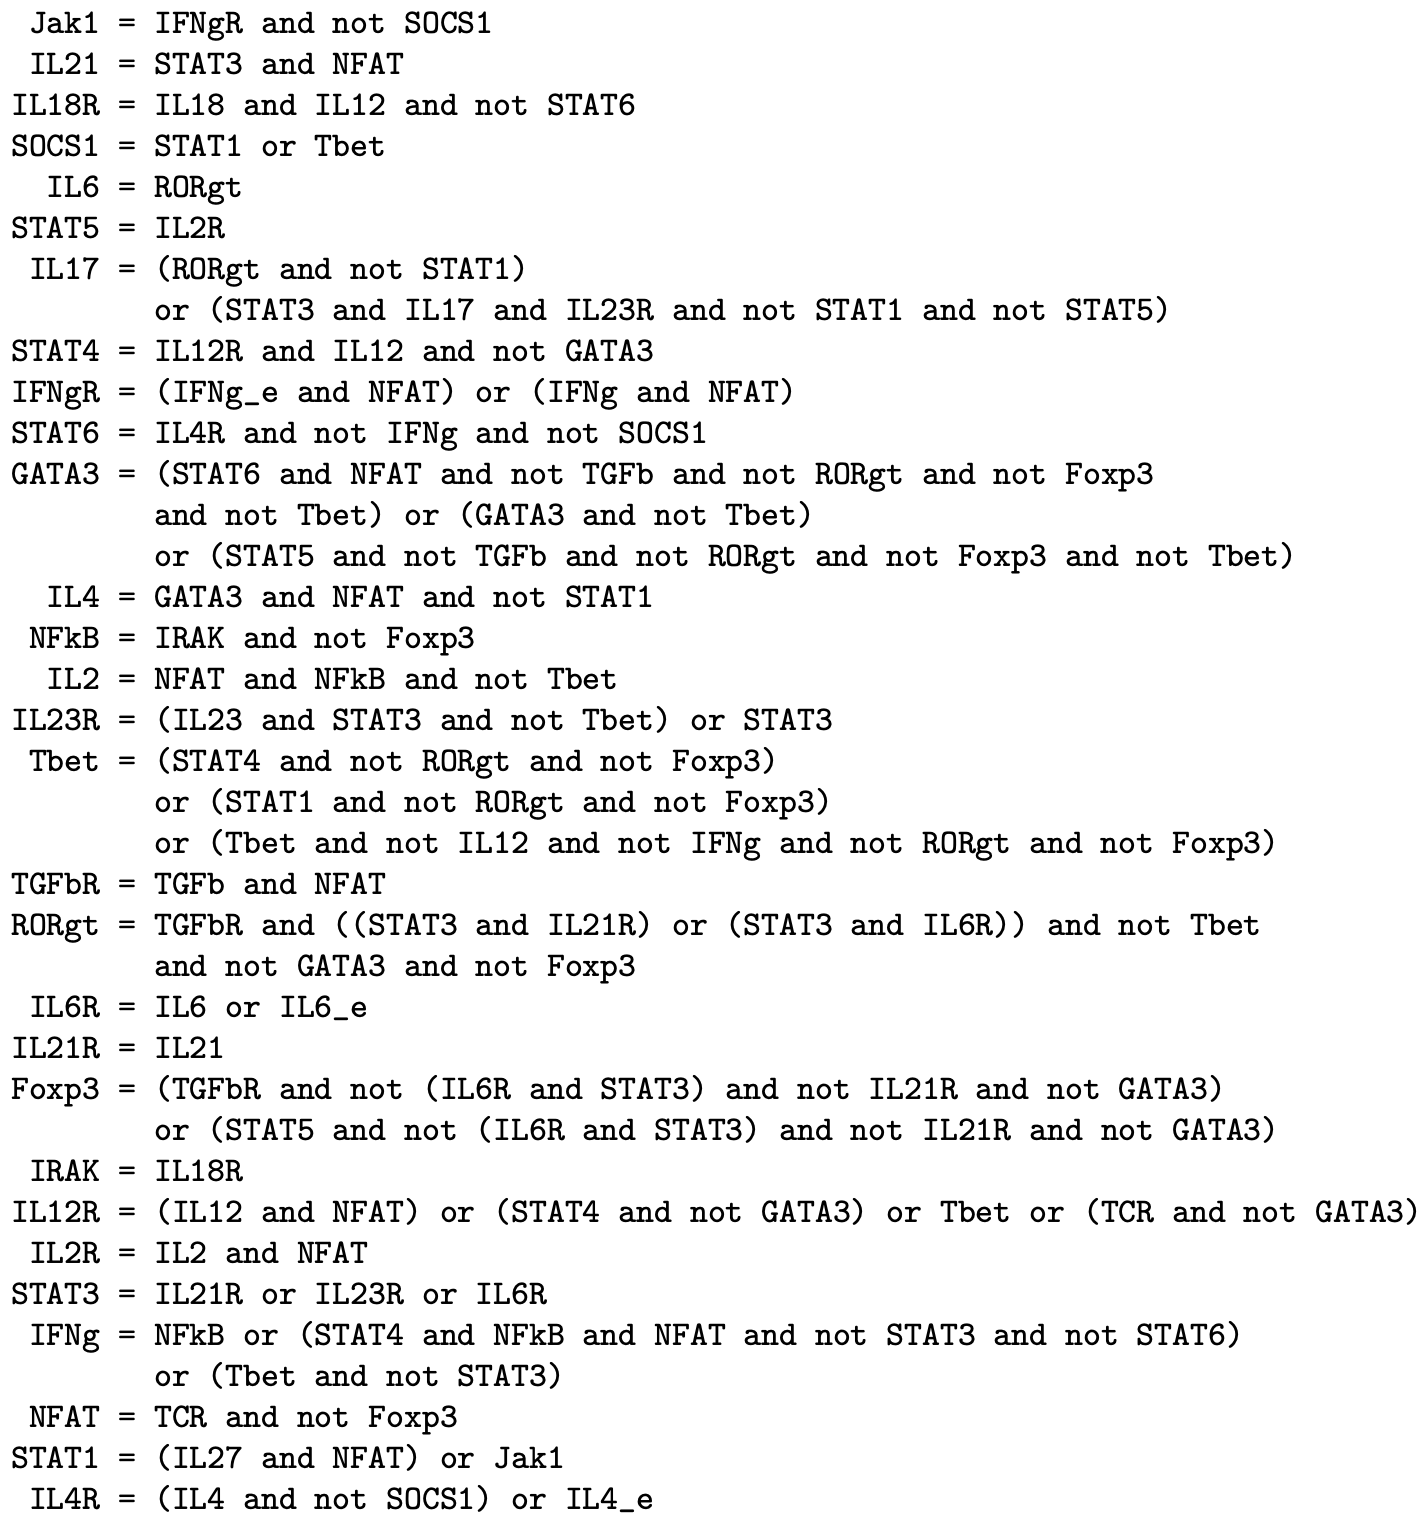
\includegraphics[width=0.49\textwidth]{figs-datamod2023/TcellBN.png}
	\end{center}
%\fontsize{8}{8}
%\begin{verbatim}
% Jak1 = IFNgR and not SOCS1 
% IL21 = STAT3 and NFAT
%IL18R = IL18 and IL12 and not STAT6 
%SOCS1 = STAT1 or Tbet 
%  IL6 = RORgt 
%STAT5 = IL2R 
% IL17 = (RORgt and not STAT1) 
%        or (STAT3 and IL17 and IL23R and not STAT1 and not STAT5) 
%STAT4 = IL12R and IL12 and not GATA3 
%IFNgR = (IFNg_e and NFAT) or (IFNg and NFAT) 
%STAT6 = IL4R and not IFNg and not SOCS1 
%GATA3 = (STAT6 and NFAT and not TGFb and not RORgt and not Foxp3 
%        and not Tbet) or (GATA3 and not Tbet) 
%        or (STAT5 and not TGFb and not RORgt and not Foxp3 and not Tbet) 
%  IL4 = GATA3 and NFAT and not STAT1 
% NFkB = IRAK and not Foxp3 
%  IL2 = NFAT and NFkB and not Tbet 
%IL23R = (IL23 and STAT3 and not Tbet) or STAT3 
% Tbet = (STAT4 and not RORgt and not Foxp3) 
%        or (STAT1 and not RORgt and not Foxp3) 
%        or (Tbet and not IL12 and not IFNg and not RORgt and not Foxp3) 
%TGFbR = TGFb and NFAT 
%RORgt = TGFbR and ((STAT3 and IL21R) or (STAT3 and IL6R)) and not Tbet 
%        and not GATA3 and not Foxp3 
% IL6R = IL6 or IL6_e 
%IL21R = IL21 
%Foxp3 = (TGFbR and not (IL6R and STAT3) and not IL21R and not GATA3) 
%        or (STAT5 and not (IL6R and STAT3) and not IL21R and not GATA3) 
% IRAK = IL18R 
%IL12R = (IL12 and NFAT) or (STAT4 and not GATA3) or Tbet or (TCR and not GATA3) 
% IL2R = IL2 and NFAT 
%STAT3 = IL21R or IL23R or IL6R 
% IFNg = NFkB or (STAT4 and NFkB and NFAT and not STAT3 and not STAT6) 
%        or (Tbet and not STAT3) 
% NFAT = TCR and not Foxp3 
%STAT1 = (IL27 and NFAT) or Jak1 
% IL4R = (IL4 and not SOCS1) or IL4_e 
%\end{verbatim}
	\caption{Boolean updates of the T Cell differentiation model from \cite{puniya2018mechanistic}, available at \cite{ModelCellCollective}.}
	\label{fig:boolean-formulas}
\end{figure}

\begin{figure}[t]
\begin{minipage}{0.9\linewidth}
\footnotesize
\begin{verbatim}
myreactions([
    react([stat5],[gata3,il21r,il6r],[foxp3]),
    react([stat5],[gata3,il21r,stat3],[foxp3]),
    react([tgfbr],[gata3,il21r,il6r],[foxp3]),
    react([tgfbr],[gata3,il21r,stat3],[foxp3]),
    react([gata3],[tbet],[gata3]),
    react([nfat,stat6],[foxp3,rorgt,tbet,tgfb],[gata3]),
    react([stat5],[foxp3,rorgt,tbet,tgfb],[gata3]),
    react([nfat,nfkb,stat4],[stat3,stat6],[ifng]),
    react([nfkb],[],[ifng]),
    react([tbet],[stat3],[ifng]),
    react([ifng,nfat],[],[ifngr]),
    react([ifnge,nfat],[],[ifngr]),
    react([il12,nfat],[],[il12r]),
    react([tbet],[],[il12r]),
    react([tcr],[gata3],[il12r]),
    react([il17,il23r,stat3],[stat1,stat5],[il17]),
    react([rorgt],[stat1],[il17]),
    react([il12,il18],[stat6],[il18r]),
    react([nfat,nfkb],[tbet],[il2]),
    react([nfat,stat3],[],[il21]),
    react([il21],[],[il21r]),
    react([il23,stat3],[tbet],[il23r]),
    react([stat3],[],[il23r]),
    react([il2,nfat],[],[il2r]),
    react([stat4],[gata3],[il2r]),
    react([gata3,nfat],[stat1],[il4]),
    react([il4],[socs1],[il4r]),
    react([il4e],[],[il4r]),
    react([rorgt],[],[il6]),
    react([il6],[],[il6r]),
    react([il6e],[],[il6r]),
    react([il18r],[],[irak]),
    react([ifngr],[socs1],[jak1]),
    react([tcr],[foxp3],[nfat]),
    react([irak],[foxp3],[nfkb]),
    react([il21r,stat3,tgfbr],[foxp3,gata3,tbet],[rorgt]),
    react([il6r,stat3,tgfbr],[foxp3,gata3,tbet],[rorgt]),
    react([stat1],[],[socs1]),
    react([tbet],[],[socs1]),
    react([il27,nfat],[],[stat1]),
    react([jak1],[],[stat1]),
    react([il21r],[],[stat3]),
    react([il23r],[],[stat3]),
    react([il6r],[],[stat3]),
    react([il12,il12r],[gata3],[stat4]),
    react([il2r],[],[stat5]),
    react([il4r],[ifng,socs1],[stat6]),
    react([stat1],[foxp3,rorgt],[tbet]),
    react([stat4],[foxp3,rorgt],[tbet]),
    react([tbet],[foxp3,ifng,il12,rorgt],[tbet]),
    react([nfat,tgfb],[],[tgfbr]) ]).
    
\end{verbatim}
\end{minipage}
\caption{\BioResolve implementation of the T cell case study from \Cref{sec:datamod2023}.}
\label{fig:bioresolve:tcell}
\end{figure}


